\section{Specyfikacja sprzętu oraz oprogramowania podstawowego}

System zostanie zrealizowany w architekturze trójwarstwowej. Będzie składał się z następujących warstw:

\begin{itemize}
	\item[--] warstwa prezentacji (interfejs użytkownika),
	\item[--] warstwa logiki biznesowej (pośrednicząca w dostępie do danych zapisanych w bazie danych),
	\item[--] warstwa danych.
\end{itemize}

\subsection{Warstwa prezentacji}

Warstwa prezentacji będzie elementem odpowiedzialnym za prezentację treści użytkownikowi końcowemu. Będzie również umożliwiać odbieranie żądań użytkowników i przesyłanie ich do kolejnych warstw. Dzięki obecności warstwy prezentacji użytkownicy naszego systemu nie są zobowiązani do przeprowadzania instalacji dodatkowego oprogramowania w celu korzystania z jego możliwości - jedynym wymogiem jest posiadanie przeglądarki internetowej, za pomocą której użytkownik będzie logował się do systemu.

\subsection{Warstwa logiki biznesowej}

Warstwa logiki biznesowej będzie składać się ze zbioru komponentów odpowiedzialnych za
spełnianie poszczególnych założeń funkcjonalnych systemu (o których mowa w niniejszym dokumencie).

\subsection{Warstwa danych}

Warstwa danych odpowiedzialna będzie za dostęp do bazy danych - odczytywanie i zapisywanie w niej informacji.

\begin{figure}[h!]
	\centering
	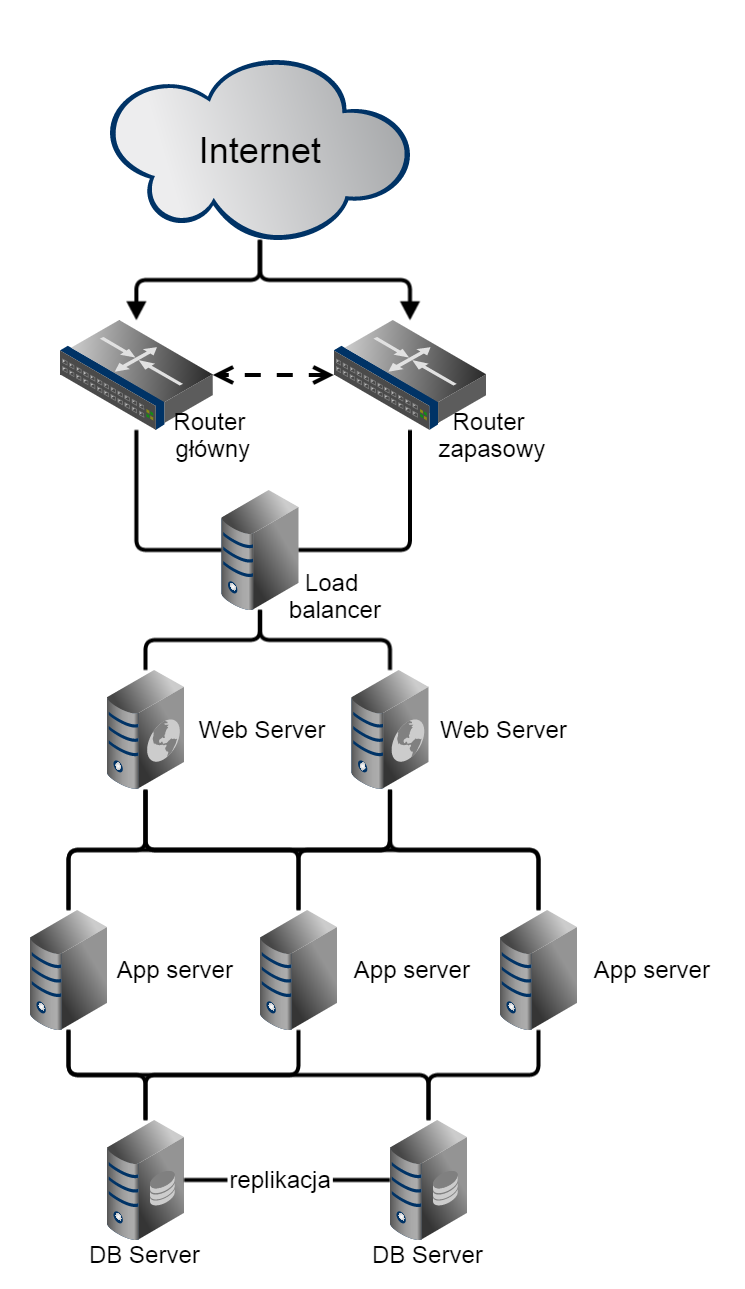
\includegraphics[scale=0.4]{img/architektura}
	\caption{Schemat architektury \label{fig:labelArchitecture}}
\end{figure}

\subsection{Schemat architektury}

Jak uwidoczniono na \ref*{fig:labelArchitecture} na wejściu żądania będą obsługiwany przez router główny, któremu towarzyszył będzie router zapasowy w przypadku, kiedy router główny nie będzie w stanie obsłużyć żądania. Następnie wybierany będzie Web Server, który będzie obsługiwał zgłoszenie (w zależności od poziomu obciążenia serwerów, decydować o tym będzie Load Balancer). W analogiczny sposób wybierany będzie serwer aplikacyjny, pośredniczący w obsłudze.

W odniesieniu do serwerów bazy danych zastosowany będzie mechanizm replikacji danych, który ma zagwarantować bezpieczeństwo przechowywanych informacji (ochronę przed ich utratą w wyniku awarii jednego z serwerów).

\subsection{Oszacowanie rozmiarów systemu}

W chwili obecnej firma posiada w ewidencji:

\begin{itemize}
\item[--] około 50 pojazdów
\item[--] około 800 telefonów
\item[--] około 1500 komputerów stacjonarnych
\item[--] około 2500 monitorów komputerowych
\item[--] około 2000 laptopów
\item[--] około 100 serwerów
\item[--] około 200 sztuk sprzętu serwerowego
\item[--] około 10000 sztuk innego drobnego sprzętu komputerowego
\item[--] około 300 nośników z oprogramowaniem
\item[--] około 200 licencji na użytkowanie oprogramowania (jedna licencja na wiele stanowisk)
\end{itemize}

Oznacza to, że w ewidencji firmy jest ponad 17 tysięcy przedmiotów i
licencji na oprogramowanie. Ponieważ firma się intensywnie rozwija
należy założyć, że system będzie obsługiwał co najmniej 30 tysięcy
przedmiotów. W chwili obecnej firma zatrudnia około 1500
pracowników. Ponieważ firma przeżywa intensywny rozwój konieczne jest
zwymiarowanie systemu na poziomie co najmnije dwukrotności obecnego
zatrudnienia to jest 3000 pracowników. System należy do grupy systemów
wspierających funkcjonowanie przedsiębiorstwa i nie będzie
wykorzystywany w ramach podstawowych zadania pracowników. Należy zatem
założyć, że nie wszyscy pracownicy będą go używali w tym samym
czasie. W związku z tym należy założyć, że równocześnie system będzie
używany przez około 10\% pracowników czyli 300 osób. Powyższe szacunki
są zgodne z wymaganiami niefunkcjonalnymi przedstawionymi w
\ref{wymagania_niefunkcjonalne}.

\subsection{Rozkład obciążenia na poszczególne warstwy}

Aplikacja w architekturze trójwarstwowej posiada budowę bardzo
modularną, przez co mozliwe jest rozmieszczenie różnych elementów na
odpowiednich maszynach. Dzięki takiemu rozmieszczeniu każda z warstw
moze być wykonywana na sprzęcie dostosowanym do jej zadań. Ponieważ
każda warstwa wykonuje inne zadania to znacząco też różni się
charakterystyka sprzętu, który należy wykorzystać w danej warstwie.

\subsubsection{Warstwa prezentacji}

Warstwa prezentacji odpowiedzialna jest za wyświetlanie użytkownikowi
treści. Implementacja tej warstwy zostanie wykonana z użyciem języka
JavaScript wraz z technologiami HTML oraz CSS. Ponadto dodatkowa
funkcjonalność zostanie zaimplementowana przy użyciu biblioteki
jQuerry. Pomimo, iż zarówno serwer jak i klienci znajdować się będą w
sieci wewnętrznej przedsiębiorstwa należy zapewnić odpowiedni poziom
bezpieczeństwa poprzez wykorzystanie protokołu SSL/TLS.

Z perspektywy wymaganych zasobów sprzętowych wymagania dla tej warstwy
mozna podzielić na dwie części. Pierwsza z nich dotyczy wymagań co do
urządzenia na którym treść będzie prezentowana. Konieczne jest aby
takie urządzenie wyposażone było w przeglądarkę obsługującą
JavaScript. Druga część z wymagań sprzetowych dotyczy serwera www, do
którego kierowane będą rządania. Od tego urządzenia wymaga się przede
wszystkim wysokiej wydajności, krótkiego czasu odpowiedzi oraz
możliwości obsługi wielu klientów jednocześnie. Istotne jest również
zapewnienie wysokiej dostępności tego serwera.

\subsubsection{Warstwa logiki biznesowej}

Warstwa logiki biznesowej odpowiedzialna jest za przetwarzanie rządań
klienta w sposób zgodny z prawami rządzącymi organizacją. Zostanie ona
zaimplementowana w technologii J2EE. Jako serwer aplikacyjny wybrano
JBoos Application Server.

Z perspektywy wymaganych zasobów warstwa ta posiada analigoczne
wymagania jak warstwa prezentacji. Oznacza to, że istotna dostępność,
krótki czas odpowiedzi oraz możliwość obsługi wielu klientów
równocześnie. Te abstrakcyjne wymagania tej warstwy na sprzęt
przekładają się na duże zapotrzebowanie na procesor (w tym ich
liczbę), rozmiar pamięci RAM oraz szybkość odpowiedzi dysku twardego,
notomiast już sam rozmiar tego dysku może być nie zbyt duży.

\subsubsection{Warstwa danych}

Warstwa danych odpowiedzialna jest za przetwarzanie i przechowywanie
danych w sposób zapewniający ich spójność oraz trwałość. W tej
warstwie zostanie wykorzystana technologia Oracle DataBase 12c w
wersji Enterprise Edition. Jest to najnowsza wersja bazy danych od
Oracle i posiada wiele zaawansowanych mechanizmów, wpływających na
wydajność jak i bezpieczeństwo przechowywanych danych.

Z perspektywy wymaganych zasobów sprzętowych warstwa ta posiada
analogiczne wymagania co poprzednia lecz są one tutaj bardziej
krytyczne, gdyż zbyt długie przetwarzanie zapytania przez bazę danych
znacząco wydłuża czas odpowiedzi aplikacji. Neleży również pamietać o
dostosowaniu rozmiaru pamieci operacyjnej oraz zamontowaniu
odpowedniej liczby wydajnych dysków twardych wraz z zapewnieniem ich
replikacji w celu zabezpieczenia się przed utrata danych.

\subsection{Sprzęt}


